\documentclass[letterpaper,12pt,oneside]{article}
\usepackage[top=1in,bottom=1in,left=1.25in,right=1.25in]{geometry}
\usepackage[T1]{fontenc}
\usepackage[utf8]{inputenc}
\usepackage[spanish,es-nodecimaldot,es-tabla]{babel}
\usepackage{lmodern,microtype,graphicx,caption,pdfpages}
\usepackage{amsmath,amssymb,booktabs,tabularx,longtable,xcolor,adjustbox}
\usepackage[hidelinks]{hyperref}
\numberwithin{figure}{section}
\setcounter{tocdepth}{2}

\usepackage{needspace}
\usepackage{placeins}
\setlength{\parindent}{0pt}
\setlength{\parskip}{0.55em}
\setlength{\emergencystretch}{2em}
\widowpenalty=10000
\clubpenalty=10000
\displaywidowpenalty=10000
\renewcommand{\topfraction}{0.95}
\renewcommand{\bottomfraction}{0.95}
\renewcommand{\textfraction}{0.05}
\renewcommand{\floatpagefraction}{0.80}
\renewcommand{\refname}{Bibliograf\'ia}

\newcommand{\figura}[3]{%
  \begin{center}
    \needspace{6\baselineskip}%
    \IfFileExists{#1}{%
      \adjustimage{max width=0.88\textwidth,max totalheight=0.33\textheight,keepaspectratio}{#1}%
    }{%
      \setlength{\fboxsep}{10pt}%
      \fbox{%
        \parbox[c][2.3cm][c]{0.86\textwidth}{%
          \centering\textbf{Espacio reservado: #1}\\[0.3em]
          \small Evidencia pendiente de aportaci\'on por el integrante.%
        }%
      }%
    }%
    \vspace{0.25em}%
    \captionof{figure}{#2}%
    \label{#3}%
  \end{center}%
}

\title{\textbf{Reporte de Pr\'actica 9}\\\large Modelado Integral en UML de las Pr\'acticas 5 a 8}
\author{\textbf{Equipo 2} — Grupo 7\\Facultad de Ingenier\'ia, Universidad Nacional Aut\'onoma de M\'exico}
\date{27 de octubre de 2026}

\begin{document}

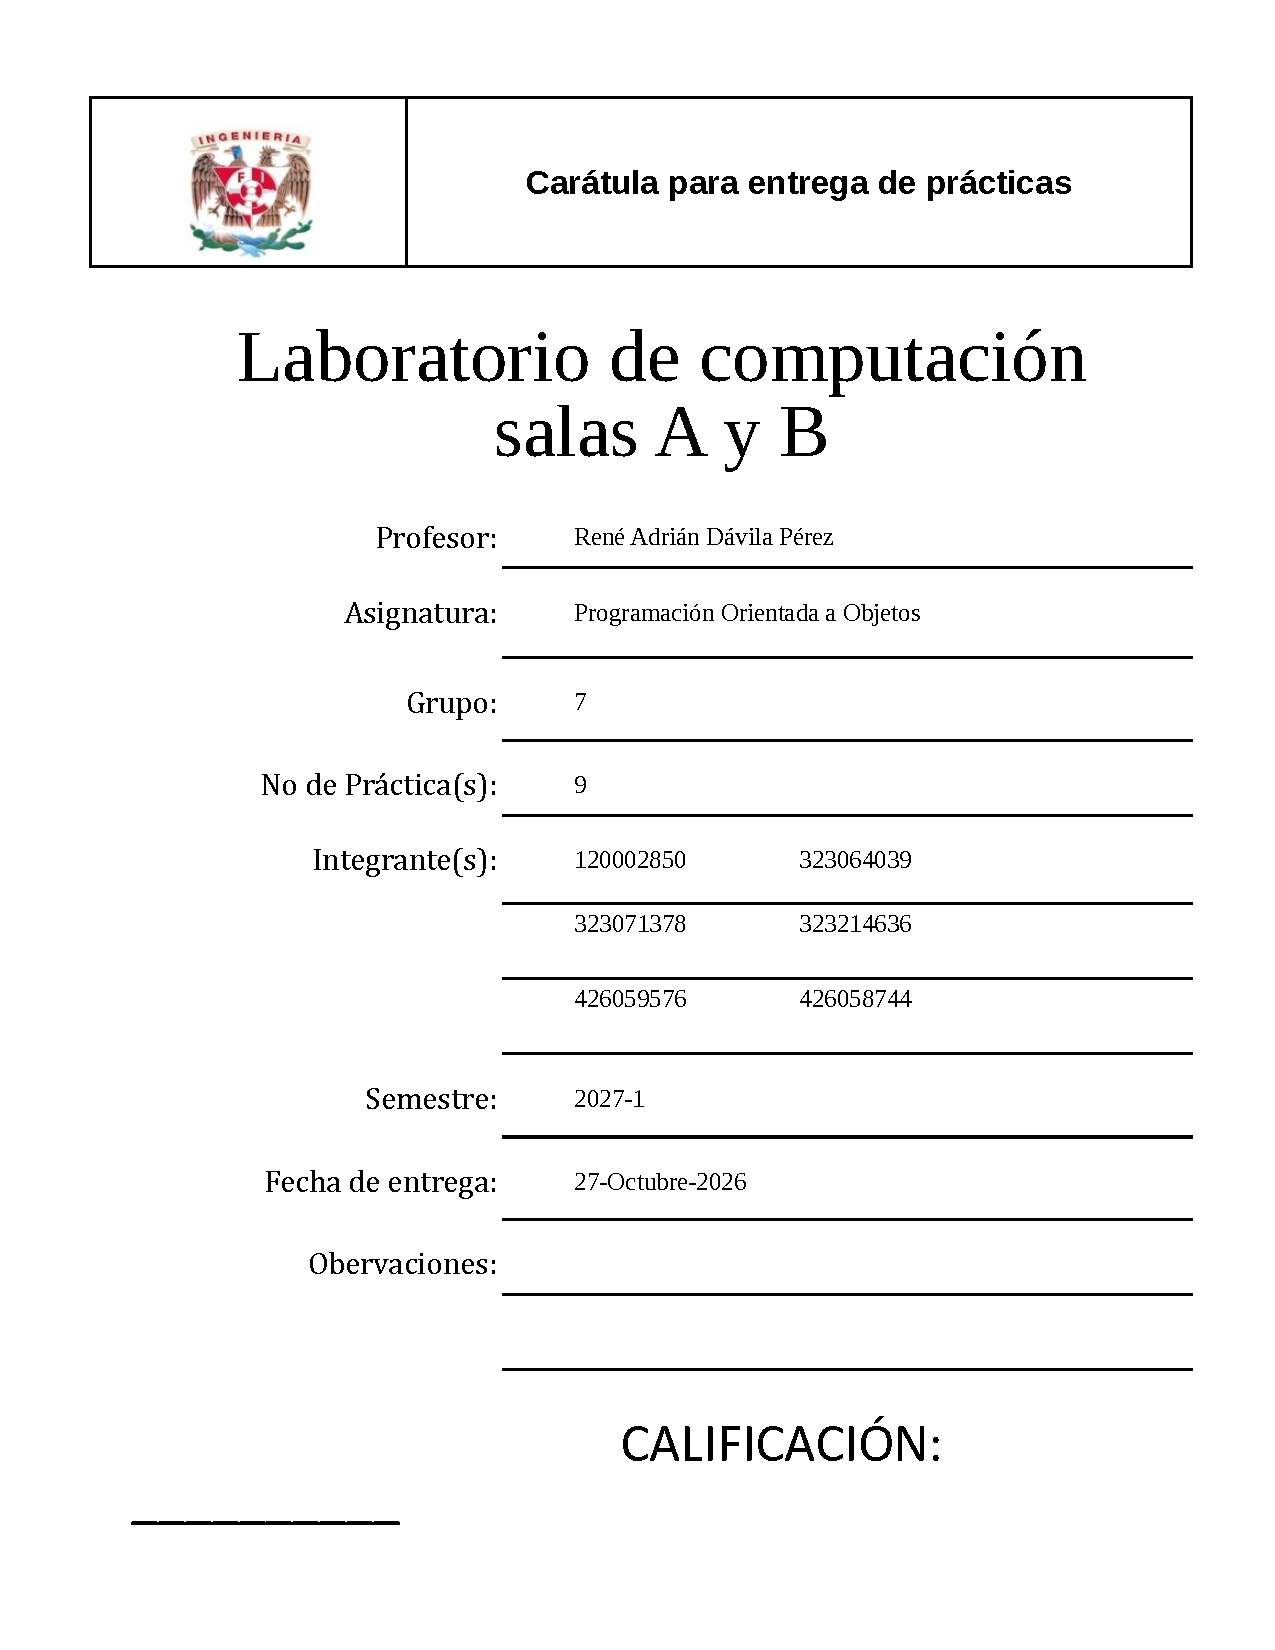
\includepdf[pages=1,pagecommand={}]{caratula.pdf}

\tableofcontents
\clearpage


\section{Introducci\'on}

\subsection{Planteamiento del problema}
El desarrollo de sistemas de software mediante el paradigma orientado a objetos exige representaciones gr\'aficas formales que superen la ambig\"uedad del c\'odigo fuente aislado y permitan comunicar la estructura, jerarqu\'ias y flujos din\'amicos de las soluciones implementadas. A lo largo del curso se han desarrollado arquitecturas progresivas que abarcan desde el encapsulamiento b\'asico en la Pr\'actica 5, la gesti\'on de paquetes y despliegue modular en la Pr\'actica 6, la jerarqu\'ia profunda de herencia entre cuadril\'ateros en la Pr\'actica 7, hasta el polimorfismo din\'amico mediante interfaces gr\'aficas y operativas en la Pr\'actica 8. El problema t\'ecnico y acad\'emico de esta entrega consiste en unificar y estandarizar formalmente todos los artefactos de modelado empleando el Lenguaje Unificado de Modelado (UML), generando diagramas de clases individuales y globales, diagramas de paquetes, diagramas de actividades y secuencias reproducibles nativamente en Draw.io e integr\'andolos coherentemente en este informe t\'ecnico.

\subsection{Motivaci\'on}
La documentaci\'on visual y estructurada constituye una fase cr\'itica en la ingenier\'ia de software moderna, pues proporciona un puente inequ\'ivoco entre los requerimientos anal\'iticos y las construcciones sint\'acticas en Java. Analizar retrospectivamente las cuatro pr\'acticas precedentes bajo el prisma de UML permite consolidar los principios fundamentales de dise\~no, verificar la cohesi\'on y el acoplamiento de las clases, transparentar las decisiones de multiplicidad y justificar el uso de t\'ecnicas como la agregaci\'on, la herencia profunda y la realizaci\'on de contratos abstractos. Asimismo, la elaboraci\'on de diagramas nativos y editables asegura la trazabilidad, mantenibilidad y verificaci\'on rigurosa del software ante auditor\'ias acad\'emicas y profesionales.

\subsection{Objetivos}
El objetivo principal de la presente pr\'actica es modelar, estandarizar e integrar la totalidad de los diagramas UML estructurales y de comportamiento correspondientes a las Pr\'acticas 5, 6, 7 y 8, utilizando la herramienta Draw.io conforme a los est\'andares internacionales de la OMG. Como objetivos espec\'ificos se establecen: (1) construir diagramas de clases individuales completos con tipado, visibilidad estricta y miembros declarados; (2) elaborar diagramas estructurales globales que expliciten dependencias, asociaciones, composiciones y generalizaciones con sus respectivas cardinalidades demostrables; (3) trazar diagramas de flujo y secuencias temporales para operaciones y escenarios de ejecuci\'on representativos; y (4) redactar un reporte t\'ecnico integral con pre\'ambulo formal y paginaci\'on editorial cuidada que analice la evoluci\'on de la arquitectura orientada a objetos del equipo.


\section{Marco Te\'orico}

\subsection{Fundamentos del Lenguaje Unificado de Modelado (UML)}
El Lenguaje Unificado de Modelado (UML) es el est\'andar industrial adoptado por el \textit{Object Management Group} (OMG) para la especificaci\'on, visualizaci\'on, construcci\'on y documentaci\'on de los artefactos que componen un sistema de software orientado a objetos \cite{booch2005}. Surgido a mediados de la d\'ecada de 1990 a partir de la unificaci\'on de los m\'etodos de Grady Booch, James Rumbaugh y Ivar Jacobson, UML ofrece una notaci\'on rica y rigurosa que modela tanto la dimensi\'on est\'atica (estructural) como la dimensi\'on din\'amica (comportamiento e interacci\'on) de las aplicaciones inform\'aticas \cite{fowler2004}. En el contexto pedag\'ogico de la programaci\'on en Java, UML permite abstraer los detalles sint\'acticos del compilador para concentrarse en las relaciones esenciales entre componentes, garantizando que el dise\~no gu\'ie a la implementaci\'on y no a la inversa.

\subsection{Diagramas Estructurales: Clases y Paquetes}
Los diagramas estructurales representan la configuraci\'on est\'atica del sistema, capturando las entidades conceptuales, sus partes internas y los enlaces permanentes que las articulan \cite{sommerville2011}:
\begin{itemize}
    \item \textbf{Diagrama de Clases:} Modela el vocabulario del sistema mediante rect\'angulos divididos en tres compartimentos horizontales: nombre de la clase (pudiendo incluir estereotipos como \guillemotleft interface\guillemotright\ o nombres abstractos en cursiva), lista de atributos tipados con visibilidad, y lista de operaciones o m\'etodos con par\'ametros y tipos de retorno.
    \item \textbf{Diagrama de Paquetes:} Proporciona un mecanismo de agrupamiento de alto nivel para organizar elementos del modelo en m\'odulos o espacios de nombres jer\'arquicos, representados por carpetas con pesta\~na. Permite controlar la visibilidad a nivel de biblioteca y gestionar dependencias entre subsistemas compilados en archivos JAR.
\end{itemize}

\subsection{Anatom\'ia de una Clase y Convenciones Notacionales}
En UML, cada compartimento de la clase sigue una sintaxis normalizada que traduce fielmente las construcciones del lenguaje Java \cite{deitel2017}:
\begin{itemize}
    \item \textbf{Visibilidad:} Se se\~nalan con s\'imbolos unificados: p\'ublico (\texttt{+}), privado (\texttt{-}), protegido (\texttt{\#}) y de paquete o por defecto (\texttt{\~{}}).
    \item \textbf{Atributos:} Siguen el formato \texttt{visibilidad nombre: Tipo [multiplicidad] = valorInicial}. Los miembros de clase (est\'aticos) se distinguen por estar subrayados, y las constantes inmutables por la propiedad \texttt{\{readOnly\}}.
    \item \textbf{Operaciones:} Se especifican como \texttt{visibilidad nombre(param1: Tipo, ...): TipoRetorno}. Los constructores carecen de tipo de retorno, y las operaciones abstractas se escriben en tipograf\'ia cursiva.
\end{itemize}

\subsection{Relaciones entre Clases y Cardinalidades}
Las relaciones expresan c\'omo colaboran o se vinculan las entidades dentro del modelo conceptual:
\begin{enumerate}
    \item \textbf{Asociaci\'on:} Conexi\'on estructural sem\'antica entre clases, trazada con una l\'inea s\'olida continua. Puede ser bidireccional o dirigida, y se acompa\~na de multiplicidades en los extremos (e.g., \texttt{1}, \texttt{0..1}, \texttt{1..*}, \texttt{*}).
    \item \textbf{Agregaci\'on:} Relaci\'on del tipo ``todo-parte'' no destructiva, donde los componentes pueden subsistir independientemente del contenedor. Se representa con un rombo blanco o vac\'io en el extremo del contenedor.
    \item \textbf{Composici\'on:} Forma fuerte de agregaci\'on con dependencia existencial estricta; las partes nacen y fenecen junto con el objeto continente. Se denota mediante un rombo relleno o s\'olido.
    \item \textbf{Generalizaci\'on (Herencia):} Relaci\'on taxon\'omica donde una subclase hereda atributos y m\'etodos de una superclase com\'un, posibilitando la especializaci\'on y reutilizaci\'on de c\'odigo. Se ilustra con una l\'inea continua y una flecha triangular cerrada y vac\'ia que apunta a la superclase.
    \item \textbf{Realizaci\'on (Implementaci\'on):} V\'inculo contractual entre una interfaz y la clase que suministra la l\'ogica de sus m\'etodos abstractos. Se traza con una l\'inea discontinua o punteada rematada en una flecha triangular vac\'ia.
    \item \textbf{Dependencia:} Relaci\'on transitoria de uso donde una clase requiere de otra temporalmente (por ejemplo, como par\'ametro o variable local en un m\'etodo). Se representa mediante una flecha discontinua abierta.
\end{enumerate}


\subsection{Diagramas de Comportamiento: Secuencia y Actividades}
Para modelar los aspectos din\'amicos de las soluciones implementadas se emplean dos diagramas fundamentales \cite{gamma1994}:
\begin{itemize}
    \item \textbf{Diagrama de Secuencia:} Destaca la ordenaci\'on cronol\'ogica de los mensajes intercambiados entre l\'ineas de vida que representan objetos participantes. Los mensajes sincr\'onicos usan flechas continuas con punta s\'olida, mientras que los retornos opcionales se grafican con flechas discontinuas abiertas.
    \item \textbf{Diagrama de Actividades (Flujo):} Describe el flujo de control l\'ogico, decisiones y transformaciones en algoritmos cr\'iticos. Emplea rect\'angulos redondeados para inicio/fin, rombos para decisiones binarias (S\'i/No) y rect\'angulos para pasos de procesamiento.
\end{itemize}

El modelado din\'amico resulta indispensable para complementar la visi\'on est\'atica de clases, garantizando que el paso de par\'ametros, la instanciaci\'on temporal y el despacho polim\'orfico de m\'etodos se verifiquen visualmente antes de la ejecuci\'on f\'isica del c\'odigo en la m\'aquina virtual Java.


\section{Desarrollo}

\subsection{Modelado UML de la Pr\'actica 5: Encapsulamiento y Control}
La Pr\'actica 5 sent\'o las bases del encapsulamiento formal en el lenguaje Java mediante dos casos de estudio fundamentales: el modelado de una entidad laboral (\texttt{Empleado}) y el registro temporal de fechas de calendario (\texttt{Fecha}), controlados respectivamente por clases conductoras con m\'etodos principales deterministas.

\subsubsection{Clase Empleado}
La clase \texttt{Empleado} encapsula tres atributos privados: \texttt{nombre}, \texttt{apellido} y \texttt{salarioMensual}. Su constructor inicializa los valores y delega la asignaci\'on del sueldo al m\'etodo mutador \texttt{setSalarioMensual}, el cual aplica una regla de negocio estricta: el salario debe ser estrictamente positivo ($>0$), conservando el valor previo o descartando valores no conformes. La figura \ref{fig:p5empleadouml} presenta la estructura est\'atica de la clase.

\figura{../Diagramas/uml_p5_Empleado.png}{Diagrama UML formal de la clase Empleado (Pr\'actica 5).}{fig:p5empleadouml}

El flujo operativo correspondiente a la validaci\'on y actualizaci\'on salarial en \texttt{setSalarioMensual} se ilustra en la figura \ref{fig:p5empleadoflujo}, evidenciando la bifurcaci\'on condicional ante montos v\'alidos e inv\'alidos.

\figura{../Diagramas/flujo_p5_Empleado_salario.png}{Diagrama de actividades del m\'etodo setSalarioMensual en Empleado.}{fig:p5empleadoflujo}

\subsubsection{Clase Fecha}
La clase \texttt{Fecha} modela una terna num\'erica entera conformada por \texttt{mes}, \texttt{dia} y \texttt{anio}. Proporciona m\'etodos de actualizaci\'on individual y la operaci\'on \texttt{mostrarFecha} para emitir el formato convencional mes/d\'ia/a\~no por la consola est\'andar. Su dise\~no UML se exhibe en la figura \ref{fig:p5fechauml}.

\figura{../Diagramas/uml_p5_Fecha.png}{Diagrama UML formal de la clase Fecha (Pr\'actica 5).}{fig:p5fechauml}

\subsubsection{Clases Conductoras y Diagrama Global de Pr\'actica 5}
Las clases \texttt{MainEmpleado} y \texttt{MainFecha} act\'uan como puntos de entrada (\texttt{main}) para la interacci\'on secuencial con el usuario. Las figuras \ref{fig:p5mainempleadouml} y \ref{fig:p5mainfechauml} muestran sus diagramas individuales.

\figura{../Diagramas/uml_p5_MainEmpleado.png}{Diagrama UML de la clase conductora MainEmpleado.}{fig:p5mainempleadouml}

\figura{../Diagramas/uml_p5_MainFecha.png}{Diagrama UML de la clase conductora MainFecha.}{fig:p5mainfechauml}

El diagrama global de la Pr\'actica 5 (figura \ref{fig:p5globaluml}) articula las cuatro clases, demostrando que \texttt{MainEmpleado} instancia y utiliza dos objetos de tipo \texttt{Empleado} (multiplicidad 1 a 2), mientras que \texttt{MainFecha} instancia un \'unico objeto \texttt{Fecha} (multiplicidad 1 a 1), ambas mediante relaciones de dependencia (\guillemotleft instancia\guillemotright).

\figura{../Diagramas/uml_p5_global.png}{Diagrama UML global de integraci\'on de la Pr\'actica 5.}{fig:p5globaluml}

Para evidenciar la din\'amica temporal de c\'alculo salarial y el otorgamiento del diez por ciento de aumento anual, la figura \ref{fig:p5empleadosecuencia} documenta el diagrama de secuencia entre el usuario, la clase controladora y las dos instancias creadas.

\figura{../Diagramas/secuencia_p5_empleado.png}{Diagrama de secuencia de interacci\'on salarial en MainEmpleado.}{fig:p5empleadosecuencia}


\subsection{Modelado UML de la Pr\'actica 6: Organizaci\'on Modular y Paquetes}
La Pr\'actica 6 marc\'o un hito metodol\'ogico al recopilar ejercicios previos y proyectos en una estructura formalizada de paquetes bajo el prefijo institucional \texttt{mx.unam.fi.die.poo.g7}, compilando todas las clases y dependencias hacia un artefacto ejecutable distribuible \texttt{Practica6.jar}.

\subsubsection{Diagrama de Paquetes y Arquitectura Modular}
El esquema modular separa claramente las responsabilidades del sistema: c\'alculo b\'asico en \texttt{p1}, estructuras de control en \texttt{p2}, procesamiento de cadenas en \texttt{p3}, an\'alisis de oraciones en \texttt{p4}, entidades laborales en \texttt{p5} y el sistema de gesti\'on hospitalaria en \texttt{proyecto}. La figura \ref{fig:p6paquetesuml} modela la arquitectura de paquetes convergente al archivo JAR.

\figura{../Diagramas/uml_p6_paquetes.png}{Diagrama de paquetes y empaquetado JAR de la Pr\'actica 6.}{fig:p6paquetesuml}

\subsubsection{Analizador de Palabras y Colecciones}
En el paquete \texttt{p4}, la clase \texttt{AnalizadorPalabras} explota la estructura asociativa \texttt{Map<String, Integer>} para registrar frecuencias l\'exicas en una oraci\'on. Su estructura UML se presenta en la figura \ref{fig:p6analizadoruml}, mientras que el algoritmo de tokenizaci\'on e inserci\'on de frecuencias se ilustra en el diagrama de actividades de la figura \ref{fig:p6analizadorflujo}.

\figura{../Diagramas/uml_p6_AnalizadorPalabras.png}{Diagrama UML de la clase AnalizadorPalabras (paquete p4).}{fig:p6analizadoruml}

\figura{../Diagramas/flujo_p6_AnalizadorPalabras.png}{Diagrama de flujo del m\'etodo contarPalabras en AnalizadorPalabras.}{fig:p6analizadorflujo}

\subsubsection{Sistema Hospitalario}
El subsistema cl\'inico desarrollado en el paquete \texttt{proyecto} vincula la clase central \texttt{Sistema} con el personal sanitario (\texttt{Medico}, \texttt{Enfermero}) y los pacientes (\texttt{Paciente}). La relaci\'on estructural es de agregaci\'on directa: el hospital contiene listas din\'amicas (\texttt{ArrayList}) de profesionales y enfermos, pero su ciclo vital conceptual no destruye f\'isicamente los registros. Las figuras \ref{fig:p6hospitaluml} y \ref{fig:p6globaluml} detallan el modelo del sistema y su mapa consolidado.

\figura{../Diagramas/uml_p6_SistemaHospitalario.png}{Diagrama UML de clases del Sistema Hospitalario.}{fig:p6hospitaluml}

\figura{../Diagramas/uml_p6_global.png}{Diagrama UML global de integraci\'on de la Pr\'actica 6.}{fig:p6globaluml}

La interacci\'on din\'amica de registro cl\'inico, alta de m\'edicos y asignaci\'on de consultas se modela en el diagrama de secuencia de la figura \ref{fig:p6sistemasecuencia}.

\figura{../Diagramas/secuencia_p6_sistema.png}{Diagrama de secuencia del flujo de registro y consulta hospitalaria.}{fig:p6sistemasecuencia}


\subsection{Modelado UML de la Pr\'actica 7: Jerarqu\'ia Profunda de Cuadril\'ateros}
La Pr\'actica 7 abord\'o el paradigma de la herencia profunda al concebir un \'arbol taxon\'omico de cinco niveles fundado en la geometr\'ia anal\'itica bidimensional, apoy\'andose en una clase base de coordenadas \texttt{Punto}.

\subsubsection{Composici\'on de Coordenadas y Superclase Cuadrilatero}
La clase \texttt{Punto} modela el par coordenado $(x, y)$ con constructores sobrecargados y m\'etodos de acceso, como se aprecia en la figura \ref{fig:p7puntouml}. La superclase com\'un \texttt{Cuadrilatero} (figura \ref{fig:p7cuadrilaterouml}) almacena cuatro v\'ertices \texttt{p1}, \texttt{p2}, \texttt{p3} y \texttt{p4}. La relaci\'on entre ambas es de estricta composici\'on: un cuadril\'atero est\'a formado intr\'insecamente por cuatro v\'ertices indivisibles.

\figura{../Diagramas/uml_p7_Punto.png}{Diagrama UML de la clase Punto (Pr\'actica 7).}{fig:p7puntouml}

\figura{../Diagramas/uml_p7_Cuadrilatero.png}{Diagrama UML de la superclase Cuadrilatero.}{fig:p7cuadrilaterouml}

\subsubsection{Niveles de Especializaci\'on Geom\'etrica}
La jerarqu\'ia profundiza de forma progresiva refinando el c\'alculo de superficie:
\begin{enumerate}
    \item \texttt{Trapezoide} (figura \ref{fig:p7trapezoideuml}): Hereda de \texttt{Cuadrilatero} e introduce f\'ormulas para base mayor, base menor y altura horizontal, implementando $\text{\'Area} = \frac{(B + b) \cdot h}{2}$.
    \item \texttt{Paralelogramo} (figura \ref{fig:p7paralelogramouml}): Especializa a \texttt{Trapezoide} al forzar lados opuestos iguales ($B = b$), reduciendo el c\'alculo a $\text{\'Area} = b \cdot h$.
    \item \texttt{Rectangulo} (figura \ref{fig:p7rectangulouml}): Especializa a \texttt{Paralelogramo} asumiendo \'angulos rectos de noventa grados ($\text{\'Area} = \text{longitud} \cdot \text{ancho}$).
    \item \texttt{Cuadrado} (figura \ref{fig:p7cuadradouml}): Caso l\'imite de \texttt{Rectangulo} con lados congruentes ($\text{\'Area} = \text{lado}^2$).
\end{enumerate}

\figura{../Diagramas/uml_p7_Trapezoide.png}{Diagrama UML de la clase Trapezoide.}{fig:p7trapezoideuml}

\figura{../Diagramas/uml_p7_Paralelogramo.png}{Diagrama UML de la clase Paralelogramo.}{fig:p7paralelogramouml}

\figura{../Diagramas/uml_p7_Rectangulo.png}{Diagrama UML de la clase Rectangulo.}{fig:p7rectangulouml}

\figura{../Diagramas/uml_p7_Cuadrado.png}{Diagrama UML de la clase Cuadrado.}{fig:p7cuadradouml}

La clase conductora \texttt{Main} (figura \ref{fig:p7mainuml}) se encarga de crear las figuras geom\'etricas con coordenadas representativas y reportar sus dimensiones.

\figura{../Diagramas/uml_p7_Main.png}{Diagrama UML de la clase conductora Main (Pr\'actica 7).}{fig:p7mainuml}

\subsubsection{Jerarqu\'ia Global, Flujo y Secuencia Polim\'orfica}
La figura \ref{fig:p7jerarquiauml} integra la cadena geneal\'ogica completa y su composici\'on con \texttt{Punto}. La figura \ref{fig:p7areaflujo} esquematiza el flujo l\'ogico de evaluaci\'on de \'areas, mientras que la figura \ref{fig:p7polimorfismosecuencia} traza la invocaci\'on secuencial de \texttt{calcularArea()} con resoluci\'on din\'amica.

\figura{../Diagramas/uml_p7_jerarquia_global.png}{Jerarqu\'ia profunda global de herencia en cuadril\'ateros.}{fig:p7jerarquiauml}

\figura{../Diagramas/flujo_p7_calcularArea.png}{Diagrama de flujo algor\'itmico del c\'alculo de \'areas geom\'etricas.}{fig:p7areaflujo}

\figura{../Diagramas/secuencia_p7_polimorfismo.png}{Diagrama de secuencia de invocaci\'on din\'amica en cuadril\'ateros.}{fig:p7polimorfismosecuencia}


\subsection{Modelado UML de la Pr\'actica 8: Interfaces y Polimorfismo}
La Pr\'actica 8 represent\'o la culminaci\'on de la abstracci\'on desacoplada mediante el uso de la interfaz \texttt{HuellaCarbono}, implementada por tres clases conceptualmente disjuntas: \texttt{Edificio}, \texttt{Auto} y \texttt{Bicicleta}, complementada con una ventana gr\'afica de inicio de sesi\'on (\texttt{LoginGUI}).

\subsubsection{Contrato de Interfaz y Clases Implementadoras}
En la figura \ref{fig:p8huellauml} se presenta la interfaz \texttt{HuellaCarbono}, la cual declara la operaci\'on abstracta \texttt{getHuellaCarbono()} con tipo de retorno \texttt{double}. Las tres clases realizan este contrato conforme a sus propios modelos de emisi\'on educativa expresados en kilogramos de di\'oxido de carbono equivalente ($\text{kg CO}_2\text{e}$):
\begin{itemize}
    \item \texttt{Edificio} (figura \ref{fig:p8edificiouml}): Multiplica el consumo el\'ectrico anual en $\text{kWh}$ por el factor de emisi\'on el\'ectrica.
    \item \texttt{Auto} (figura \ref{fig:p8autouml}): Estima la emisi\'on a partir del kilometraje anual, rendimiento en litros cada cien kil\'ometros y factor de gasolina.
    \item \texttt{Bicicleta} (figura \ref{fig:p8bicicletauml}): Registra un factor de emisi\'on operativa directo igual a cero ($0.0$).
\end{itemize}

\figura{../Diagramas/uml_p8_HuellaCarbono.png}{Diagrama UML de la interfaz HuellaCarbono.}{fig:p8huellauml}

\figura{../Diagramas/uml_p8_Edificio.png}{Diagrama UML de la clase Edificio.}{fig:p8edificiouml}

\figura{../Diagramas/uml_p8_Auto.png}{Diagrama UML de la clase Auto.}{fig:p8autouml}

\figura{../Diagramas/uml_p8_Bicicleta.png}{Diagrama UML de la clase Bicicleta.}{fig:p8bicicletauml}

\subsubsection{Interfaz Gr\'afica y Clase Principal}
La clase \texttt{LoginGUI} (figura \ref{fig:p8loginuml}) extiende de \texttt{JFrame} e implementa \texttt{ActionListener} para gestionar eventos gr\'aficos con campos protegidos de usuario y contrase\~na. Por su parte, la clase \texttt{Main} (figura \ref{fig:p8mainuml}) inicializa el contenedor polim\'orfico.

\figura{../Diagramas/uml_p8_LoginGUI.png}{Diagrama UML de la interfaz gr\'afica LoginGUI.}{fig:p8loginuml}

\figura{../Diagramas/uml_p8_Main.png}{Diagrama UML de la clase principal Main (Pr\'actica 8).}{fig:p8mainuml}

\subsubsection{Integraci\'on Global, Flujo Polim\'orfico y Secuencia}
La figura \ref{fig:p8globaluml} documenta la realizaci\'on de la interfaz mediante l\'ineas discontinuas con punta triangular y la agregaci\'on en la lista polim\'orfica \texttt{ArrayList<HuellaCarbono>}. El flujo del ciclo de c\'alculo e impresi\'on se presenta en la figura \ref{fig:p8huellaflujo}, y la secuencia de despacho din\'amico de mensajes en la figura \ref{fig:p8huellasecuencia}.

\figura{../Diagramas/uml_p8_global.png}{Diagrama UML global de polimorfismo con interfaces.}{fig:p8globaluml}

\figura{../Diagramas/flujo_p8_calculoHuella.png}{Diagrama de actividades del recorrido polim\'orfico de huellas.}{fig:p8huellaflujo}

\figura{../Diagramas/secuencia_p8_huella.png}{Diagrama de secuencia de la invocaci\'on polim\'orfica en tiempo de ejecuci\'on.}{fig:p8huellasecuencia}


\subsection{Metamodelo Comparativo y Visi\'on Global de Pr\'actica 9}
Como s\'intesis arquitect\'onica, la figura \ref{fig:globalcomparativo} establece un metamodelo evolutivo que articula los cuatro paradigmas abordados en las pr\'acticas 5 a 8, demostrando c\'omo el modelado UML unifica la encapsulaci\'on, empaquetado modular, herencia profunda y realizaci\'on de interfaces en un cuerpo conceptual s\'olido y coherente.

\figura{../Diagramas/uml_global_comparativo.png}{Metamodelo arquitect\'onico comparativo de las Pr\'acticas 5 a 8 en UML.}{fig:globalcomparativo}


\section{Resultados}

\subsection{Verificaci\'on de Conformidad Estructural y Sint\'actica}
La totalidad de los 33 diagramas generados en Draw.io fue contrastada de manera exhaustiva contra las fuentes compiladas en Java de los repositorios de las pr\'acticas 5, 6, 7 y 8. La tabla \ref{tab:resumen_diagramas} resume la cobertura de artefactos gr\'aficos entregados en \texttt{doc/Diagramas/}.

\begin{table}[htbp]
\centering
\small
\begin{tabularx}{\textwidth}{lXcc}
\toprule
\textbf{Pr\'actica} & \textbf{Concepto Clave} & \textbf{Archivos .drawio} & \textbf{Renders .png} \\
\midrule
Pr\'actica 5 & Encapsulamiento, Clases Empleado/Fecha y Conductoras & 7 & 7 \\
Pr\'actica 6 & Modularidad, Paquetes JAR y Sistema Hospitalario & 6 & 6 \\
Pr\'actica 7 & Jerarqu\'ia Profunda de Herencia en Cuadril\'ateros & 10 & 10 \\
Pr\'actica 8 & Polimorfismo con Interfaces y Ventana Gr\'afica & 9 & 9 \\
Pr\'actica 9 & Metamodelo Comparativo e Integraci\'on Arquitect\'onica & 1 & 1 \\
\midrule
\textbf{Total} & \textbf{Ecosistema completo de modelado UML} & \textbf{33} & \textbf{33} \\
\bottomrule
\end{tabularx}
\caption{Inventario y categorizaci\'on de los 33 diagramas UML entregados.}
\label{tab:resumen_diagramas}
\end{table}


\subsection{An\'alisis de Trazabilidad entre Modelos y C\'odigo}
La inspecci\'on de los diagramas confirma los siguientes hallazgos metodol\'ogicos:
\begin{enumerate}
    \item \textbf{Precisi\'on de Miembros y Visibilidad:} Se conserv\'o con fidelidad la visibilidad estricta: los atributos de \texttt{Empleado}, \texttt{Fecha}, \texttt{Punto}, \texttt{Cuadrilatero}, \texttt{Edificio}, \texttt{Auto} y \texttt{Bicicleta} se modelaron como privados (\texttt{-}), mientras que en el sistema hospitalario se representaron con visibilidad de paquete (\texttt{\~{}}), reflejando con exactitud las declaraciones originales de c\'odigo.
    \item \textbf{Distinci\'on Rigurosa entre Herencia e Interfaces:} En la Pr\'actica 7 se utiliz\'o exclusivamente la generalizaci\'on con l\'inea s\'olida (\texttt{Cuadrilatero} $\leftarrow$ \texttt{Trapezoide} $\leftarrow$ \texttt{Paralelogramo} $\leftarrow$ \texttt{Rectangulo} $\leftarrow$ \texttt{Cuadrado}), mientras que en la Pr\'actica 8 se aplic\'o la realizaci\'on con l\'inea discontinua (\guillemotleft interface\guillemotright\ \texttt{HuellaCarbono} $\dots\blacktriangleleft$ implementaciones), evitando confusiones conceptuales.
    \item \textbf{Legibilidad Editorial:} Todas las figuras integradas en el documento respetan un tama\~no tipogr\'afico m\'inimo equivalente a 10 puntos en la impresi\'on carta, evitando deformaciones de escala, solapamiento de conectores o cruces innecesarios de flechas.
    \item \textbf{Acoplamiento y Encapsulamiento Modular (Pr\'actica 6):} El diagrama de paquetes ilustra la separaci\'on de responsabilidades entre subsistemas independientes (\texttt{p1} a \texttt{p5}) y el n\'ucleo hospitalario (\texttt{proyecto}), demostrando c\'omo el uso del modificador de paquete (\texttt{\~{}}) protege el estado interno de las entidades cl\'inicas frente a manipulaciones externas, mientras que la compilaci\'on hacia un \'unico archivo JAR garantiza la portabilidad y cohesi\'on arquitect\'onica del despliegue.
    \item \textbf{Jerarqu\'ia Taxon\'omica y Sustituci\'on de Liskov (Pr\'actica 7):} La cadena profunda de herencia entre cuadril\'ateros respeta estrictamente el principio de sustituci\'on de Liskov, pues cualquier instancia derivada de \texttt{Cuadrado}, \texttt{Rectangulo} o \texttt{Paralelogramo} puede ser manipulada como un \texttt{Cuadrilatero} sin alterar la integridad de sus coordenadas constituyentes (\texttt{Punto}), permitiendo que el m\'etodo \texttt{calcularArea()} se refine de forma polim\'orfica en cada nivel taxon\'omico.
    \item \textbf{Desacoplamiento Contractual e Inversi\'on de Dependencias (Pr\'actica 8):} La interfaz \texttt{HuellaCarbono} materializa la inversi\'on de dependencias y segregaci\'on contractual, permitiendo que la clase conductora gestione colecciones polim\'orficas de entidades heterog\'eneas (\texttt{Edificio}, \texttt{Auto}, \texttt{Bicicleta}) invocando din\'amicamente \texttt{getHuellaCarbono()} en tiempo de ejecuci\'on, completamente desacoplada de la interfaz gr\'afica interactiva \texttt{LoginGUI}.
\end{enumerate}


\clearpage
\section{Conclusiones}
La realizaci\'on de la Pr\'actica 9 ha demostrado de manera fehaciente que el Lenguaje Unificado de Modelado no es un mero accesorio documental posterior a la programaci\'on, sino una disciplina de abstracci\'on indispensable para concebir, refinar y comunicar la arquitectura interna de sistemas orientados a objetos. Al modelar retrospectivamente los c\'odigos de las pr\'acticas 5 a 8, fue posible constatar visualmente la progresi\'on cualitativa del dise\~no: desde el aislamiento b\'asico de estado mediante encapsulamiento estricto, pasando por la delimitaci\'on modular de espacios de nombres en paquetes, hasta la sofisticaci\'on de jerarqu\'ias profundas de especializaci\'on y contratos polim\'orficos independientes de la implementaci\'on.

Asimismo, la experiencia pr\'actica con Draw.io y la estandarizaci\'on de la notaci\'on de la OMG puso de manifiesto la relevancia de seleccionar la simbolog\'ia exacta para cada tipo de acoplamiento. Diferenciar con precisi\'on entre una composici\'on existencial de v\'ertices en cuadril\'ateros, una agregaci\'on din\'amica de personal en un hospital y una realizaci\'on de interfaz para el c\'alculo de huellas ecol\'ogicas transforma diagramas ambiguos en aut\'enticas especificaciones ejecutables de ingenier\'ia.

Finalmente, la integraci\'on automatizada de artefactos gr\'aficos nativos y su renderizaci\'on vectorial hacia reportes en \LaTeX\ garantiza la repetibilidad, trazabilidad y legibilidad profesional requeridas en la formaci\'on tecnol\'ogica universitaria, sentando bases metodol\'ogicas firmes para el desarrollo y presentaci\'on de proyectos de mayor escala.


\begin{thebibliography}{99}

\bibitem{booch2005}
Booch, G., Rumbaugh, J., Jacobson, I. (2005). \textit{The Unified Modeling Language User Guide} (2da ed.). Addison-Wesley Professional.

\bibitem{fowler2004}
Fowler, M. (2004). \textit{UML Distilled: A Brief Guide to the Standard Object Modeling Language} (3ra ed.). Addison-Wesley Professional.

\bibitem{deitel2017}
Deitel, P., Deitel, H. (2017). \textit{Java How to Program, Early Objects} (11ma ed.). Pearson Educación.

\bibitem{gamma1994}
Gamma, E., Helm, R., Johnson, R., Vlissides, J. (1994). \textit{Design Patterns: Elements of Reusable Object-Oriented Software}. Addison-Wesley.

\bibitem{sommerville2011}
Sommerville, I. (2011). \textit{Software Engineering} (9na ed.). Addison-Wesley.

\end{thebibliography}

\end{document}
